 \section{Naive Bayes}
 Given feature $ x \in \{0,1\}^{K}$, predict classes $c \in C$\\
 where:\\
 $x=x_{1},x_{2},...x_{K}$ and $x_{j}=1$ if word $j$ is in the document.\\ 
 $K$=size of vocabulary: approx 100k-500k\\

Bayes Rule:
\begin{equation}
p(c|x)=\frac{p(x|c)p(c)}{p(x)}
\end{equation}

"Naive" Independence Assumption: $x_{j}$'s are conditionally independent given class c i.e 
 \begin{equation}
 p(x|c)=\prod_{j=1}^{K}{ p(x_{j}|c)}
 \end{equation}
 
 Furthermore we assume that given class c, word occurrences are coin flips(have Bernouilli distribution) i.e
  \begin{equation}
  p(x_{j}|c)=\theta_{jc}^{x_{j}}(1-\theta_{jc})^{1-x_{j}}
  \end{equation}
 and $p(c)=\theta_{c}$.\\

 
 Putting this all together and taking logs we get:
 
 \begin{equation}
 log(p(c|x)) = \sum\limits_{j}log\big(\theta_{jc}^{x_{j}}(1-\theta_{jc})^{1-x_{j}}\big) + log \frac{\theta_{c}}{p(x)}
 \end{equation}
 \begin{equation}
 log(p(c|x)) = \sum\limits_{j}x_{j}log\frac{\theta_{jc}}{1-\theta_{jc}} +
 \sum\limits_{j} log(1-\theta_{jc}) + + log \frac{\theta_{c}}{p(x)}
 \end{equation}
 How can we compute $p(x)$? We could use $p(x)=\sum\limits_{c}p(x,c)$ but this will be cumbersome\\
 %
 Lets restrict ourselves to two classes, 0 and 1.\\
We want to compare $p(c=1|x)$ with $p(c=0|x)$.\\
Now $p(c=1|x) > p(c=0|x)$ iff $log\frac{p(c=1|x)}{p(c=0|x)} >0$
 \begin{equation}
 log\frac{p(c=1|x)}{p(c=0|x)} = log(p(c=1|x))-log(p(c=0|x))
 \end{equation}
 
 \begin{equation}
 log\frac{p(c=1|x)}{p(c=0|x)} = \sum\limits_{j}x_{j}log\frac{\theta_{j1}(1-\theta_{j0})}{\theta_{j0}(1-\theta_{j1})} +
 \sum\limits_{j} log\frac{(1-\theta_{j1})}{(1-\theta_{j0})} + log \frac{\theta_{1}}{\theta_{0}}
 \end{equation}
 
  \begin{equation}
  log\frac{p(c=1|x)}{p(c=1|x)} = w \cdot x +w _{0}
  \end{equation} 
 
 Note: We can precompute $w_{0}$ as it doesn't depend on $x$. \\
 Thus to predict class for any $x$ we simply need to calculate $w \cdot x +w _{0}$ and predict 1 iff $w \cdot x +w _{0} > 0$. This will take time proportionate to the number of unique words in the document.
 
 The next question is, how can we learn parameters $\theta_{jc}$ from the training data? As usual we use MLE\\
 Let's consider the general case of tossing a coin with probability of heads equal to $\theta$. If we flip the coin N times and observe n heads then what is the MLE for $\theta$?\\
   \begin{equation}
 P(data|\theta)=C\theta^{n}(1-\theta)^{N-n}  \textnormal{ for some constant C.}
  \end{equation}
  \begin{equation}
 \textnormal{Log-likelihood}=L=log(P(D|\theta))=logC + nlog(\theta) + (N-n)log(1-\theta)
  \end{equation}
  
  
 \begin{equation}
 \frac{\partial L}{\partial \theta}=\frac{n}{\theta} - \frac{N-n}{1-\theta}=0
 \end{equation}
  \begin{equation}
n(1-\theta)=\theta(N-n)
  \end{equation}
  \begin{equation}
  \theta=\frac{n}{N}=\textnormal{fraction of heads}
  \end{equation}
  
 
 Therefore the MLE for parameters:
   \begin{equation}
   \theta_{j1}=\frac{n_{j1}}{n_{1}}=\frac{\textnormal{No. of spam docs with word j}}{\textnormal{No. of spam docs}}
   \end{equation}
 and
    \begin{equation}
    \theta_{1}=\frac{n_{1}}{N}=\frac{\textnormal{No. of spam docs}}{\textnormal{No. of total docs}}
    \end{equation}
  %
  \textbf{Runtime analysis}\\
  $N$:Number of documents\\
  $K$: Number words in vocabulary\\
  $\bar{k}$: average number of words in a document \\
  Training time: $O(N\bar{k})$, Run through all the documents twice, once to create the dictionary and once to calculate counts.\\
  Storage: $O(K|C|)$ \\
  Naive Bayes can be updated in an online manner. As we get new data we can just update counts. No need to retrain the full model.
  
   \section{Logistic Regression}
   In Naive Bayes we got the following equation 
   
   \begin{equation}
   log\frac{p(c=1|x)}{p(c=0|x)} = w \cdot x
   \end{equation} 
    (we can incorporate the intercept $w_{0}$ into $w$ by adding a $1$ to each $x$)
   What if we started off with a predictor that has this form(linear log odds) and unknown weights.\\
  % Let $p(c=1|x)=p$. Thus $p(c=1|x)=1-p$
   
      \begin{equation}
      log\frac{p}{1-p} = w \cdot x
      \end{equation} 
    
      \begin{equation}
      \frac{p}{1-p} = e^{w \cdot x}
      \end{equation}   
   
      \begin{equation}
      p=(1-p) e^{w \cdot x}
      \end{equation} 
   
      \begin{equation}
      p(1+ e^{w \cdot x})=e^{w \cdot x}
      \end{equation}
 
       \begin{equation}
       p=\frac{1}{1+e^{-w \cdot x}}
       	\end{equation}  
   
   %insert figure of sigmoid functions:
   \begin{figure}[ht]
   	\begin{center}
   		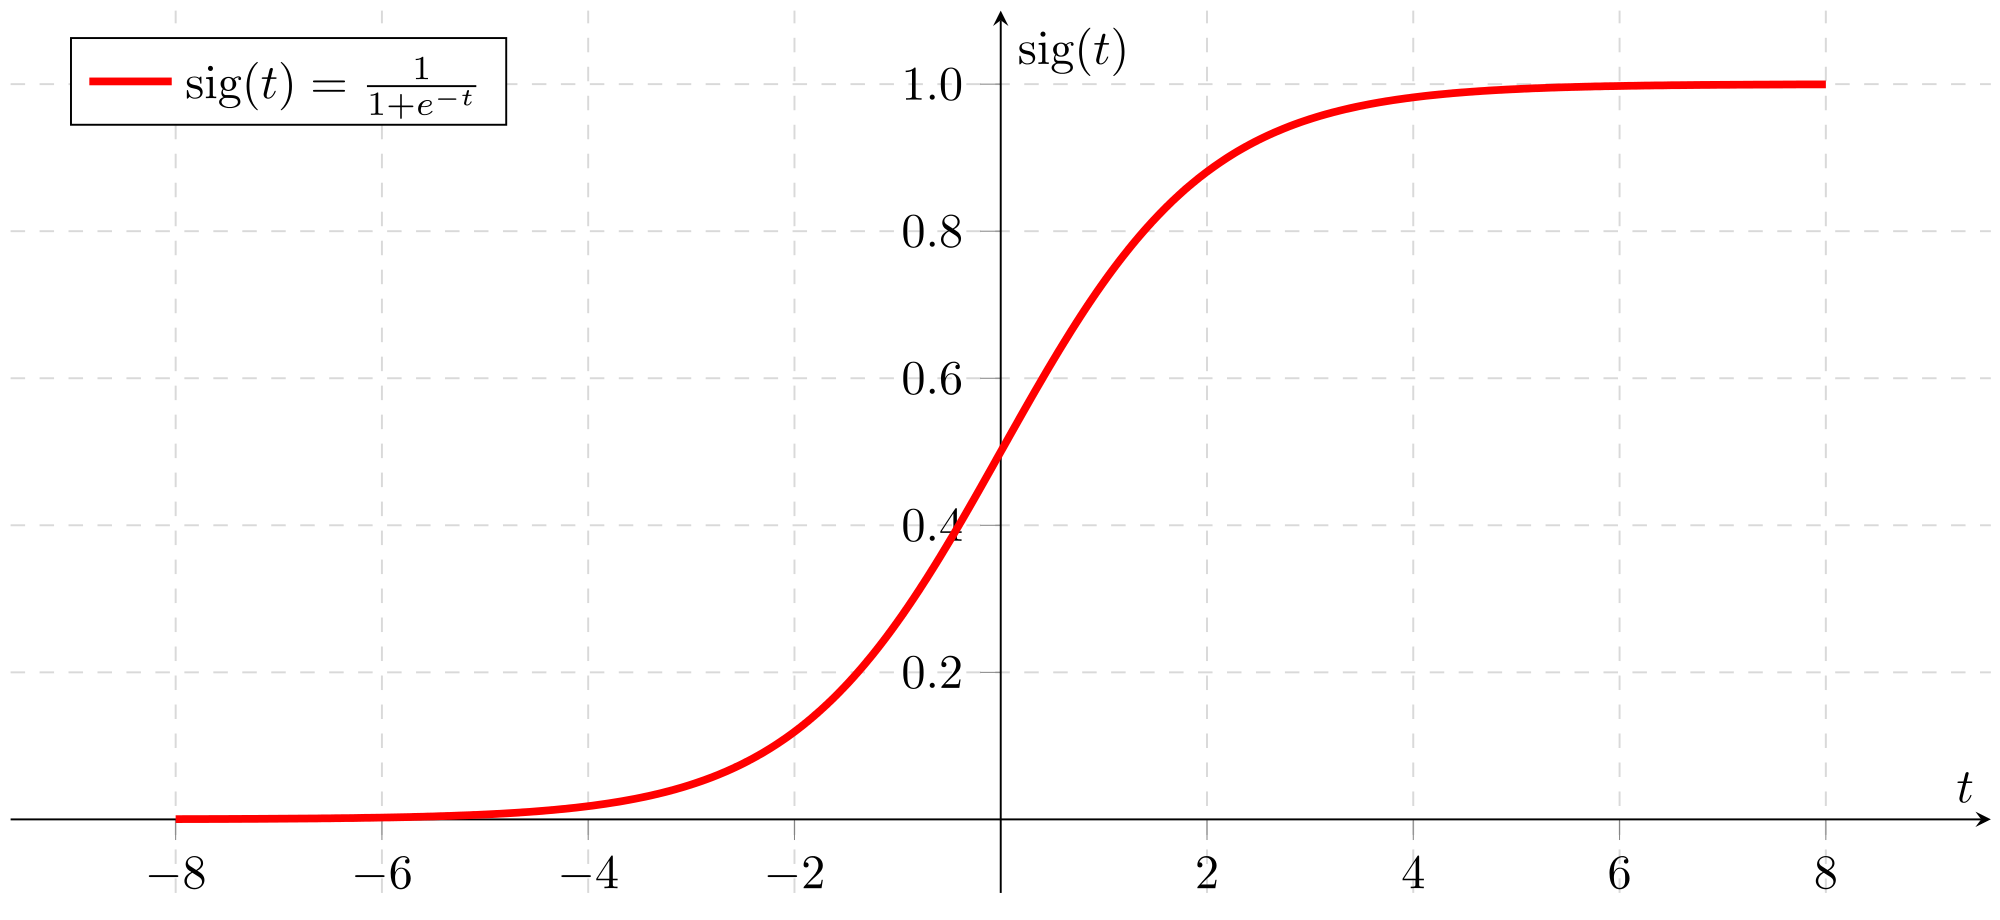
\includegraphics[width=0.5\textwidth]{figures/Sigmoid.png}
   		\caption{
   			source: https://upload.wikimedia.org/wikipedia/commons/thumb/5/53/Sigmoid-function-2.svg/2000px-Sigmoid-function-2.svg.png}
   		\label{fig:example_figure}
   	\end{center}
   \end{figure}
   
   \textbf{Key equations}:
       \begin{equation}
       p(x|w)=\frac{1}{1+e^{-w \cdot x}}
       \end{equation} 
  
       \begin{equation}
       1-p(x|w)=\frac{1}{1+e^{w \cdot x}}
       \end{equation} 
        
        \begin{equation}
        log\frac{p}{1-p} = w \cdot x
        \end{equation} 
        
        
         
        
  We have a set of documents $x_{i}$ and set of labels $y_{i}$.\\
  
    \begin{equation}
    \textnormal{Log-likelihood}=P(data|\theta)=\prod_{i}{ p_{i}^{y_{i}}(1-p_{i})^{1-y_{i}}}
    \end{equation}
    \begin{equation}
    L=-log(P(D|\theta))=-\sum\limits_{i}\{
    y_{i}logp_{i} +  (1-y_{i})log(1-p_{i})
    \}
    \end{equation}
    
    \begin{equation}
    L=-\sum\limits_{i}\{
    y_{i}log\frac{p_{i}}{{1-p_{i}}} + log(1-p_{i})
    \}
    \end{equation}
    
     \begin{equation}
     L=-\sum\limits_{i}\{
     y_{i}( w \cdot x_{i}) - log(1+e^{w \cdot x_{i}})
     \}
     \end{equation}
     
        
    \begin{equation}
    \frac{\partial L}{\partial w_{k}}=-\sum\limits_{i}\{
    y_{i}x_{ik} - \frac{1}{1+e^{w \cdot x_{i}}}e^{w \cdot x_{i}}x_{ik}
    \}=0
    \end{equation}
 
        \begin{equation}
        -\sum\limits_{i}\{(y_{i}-\frac{1}{1+e^{-w \cdot x_{i}}})x_{ik}\}=0
        \end{equation}
        
           
       \begin{equation}
       -\sum\limits_{i}\{(y_{i}-p_{i})x_{ik}\}=0
       \end{equation}
  
  Unfortunately this has no closed form solution form for w. Thus we use gradient descent.     
 
     \begin{equation}       
    w=w-\eta \frac{\partial L}{\partial w}
    \end{equation}
    \begin{equation}
     w=w + \eta X^{T}(y-p)
    \end{equation}
 or
     \begin{equation}
     w_{k}=w_{k} + \eta \sum\limits_{i}\{(y_{i}-p_{i})x_{ik}\}
     \end{equation}
 
 \subsection{Regularization}
 We can add a regularization term to the loss function.
 
     \begin{equation}
     L=-\sum\limits_{i}\{
     y_{i}logp_{i} +  (1-y_{i})log(1-p_{i})\} + \frac{1}{2}\lambda ||{w}||^{2}     
     \end{equation}
     
     \begin{equation}
     \frac{\partial L}{\partial w_{k}}=-\sum\limits_{i}\{(y_{i}-p_{i})x_{ik}\} + \lambda w_{k}
     \end{equation}
 
The gradient descent update will be
     \begin{equation}
     w_{k}=(1-\eta \lambda)w_{k} + \eta \sum\limits_{i}\{(y_{i}-p_{i})x_{ik}\}
     \end{equation}

Therefore we shrink the weight before we move against the gradient.

\section{Evaluation}
Last time\\
\textbf{Accuracy}: Fraction of time we predict the right label\\
\textbf{Calibration}: How often does an event with predicted probability p occur


\subsection{Confusion Matrix}
   %insert figure of Confusion Matrix:
   \begin{figure}[ht]
   	\begin{center}
   		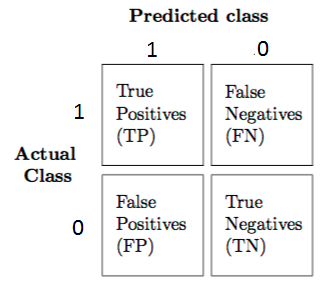
\includegraphics[width=0.5\textwidth]{figures/confusion_matrix.png}
   		\caption{
   		Confusion Matrix}
   		\label{fig:example_figure}
   	\end{center}
   \end{figure}

Thus, Accuracy=$\frac{\textnormal{TP+TN}}{\textnormal{TP+TN+FP+FN}}$\\
\\
Some other metrics:\\
\textbf{Precison}: Fraction of positive predictions that are true. i.e\\
Precison=$\frac{\textnormal{TP}}{\textnormal{TP+FP}}$ \\
\textbf{Recall/True Positive Rate}: Fraction of true examples that are predicted to be positive. i.e\\
Recall=$\frac{\textnormal{TP}}{\textnormal{TP+FN}}$ \\

In different situations we might want a model with high precision or high recall. In the case where class 1 is marking a document as spam if we want to ensure that we do not mark any email that is not spam as spam then we want a model with high precision. On the other hand if we want to ensure we get all the spam then we want a model with high recall. Another example is a situation where we want a model that classifies a manager as good or bad. If a manager is marked as bad we can take some action. If the action is strong then we want a model with high precision as it is very bad if we take an action against a manager who is in fact good(false positive). If the action is mild such as sending a mail about a management course then we want a model with high recall as it is important to ensure every bad manager gets a mail and not a big deal if a good manager gets the mail.
%
\textbf{False Positive Rate}: Fraction of false examples that are predicted to be positive. i.e\\
False Positive Rate=$\frac{\textnormal{FP}}{\textnormal{FP+TN}}$ \\


\textbf{Receiver Operator Characteristic(ROC) Curve}: Plot of True Positive Rate vs False Positive Rate
   \begin{figure}[ht]
   	\begin{center}
   		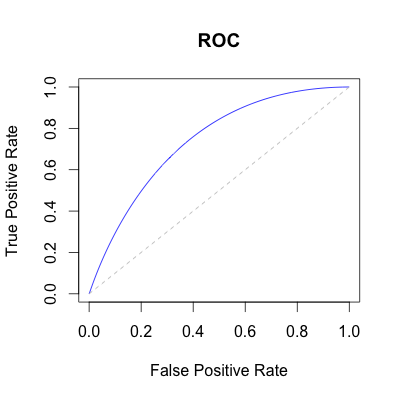
\includegraphics[width=0.5\textwidth]{figures/ROC.png}
   		\caption{source: http://danielnee.com/2014/08/area-under-the-receiver-operator-curve-auc/}
   		\label{fig:example_figure}
   	\end{center}
   \end{figure}
   
   

\textbf{Area under ROC Curve (AUC)}: Can be shown to be equivalent to accuracy for balanced classification


 \section{Computational Social Science: Exciting Progress and Future Challenges: A talk by Duncan Watts}
\textbf{Micro-macro problem}: Things studied in social sciences tend to be about collective phenomena. For example we study and try to understand entities like families, firm, political parties etc. We study them as if they are actors and have certain beliefs and preferences. This is mostly just out of convenience. In reality entities are comprised of large number of individual people who have their own beliefs, intentions and actions. The connection between micro level of individual people and macro level of social actors and facts is central to what drives social sciences.

 However this is difficult to study empirically as we need to collect data about all individuals, interactions and collective behavior. This is a daunting challenge even if we just want to observe phenomena.To study cause and effect we need to do something that resembles an experiment which is impossible.
 
 The digital revolution over the last 20 years has started to lift some of these barriers. We can now see:
 \begin{itemize}
 	\item Increase in scope, scale and granularity of data. Can obtain data from ecommerce, search websites, social media, social networks
 	\item Increase in speed and scale of experiments. Can run experiments in "virtual labs" online. Earlier restricted to mostly undergraduate students in a psychology lab for a couple of hours. 
\end{itemize}

\subsection{Study of social Contagion using "Big Data"}
Contagion implies large multi-step peer to peer spread. If we plot time on x axis and total number of adopters aggregated over population on the y axis we observer a S shaped curve. Traditionally we claim that this curve is an indicator of diffusion: there are a few early adopters, then there is an exponential increase and eventually it slows down as the entire population has adopted. However there are 2 problems with this argument:
 \begin{itemize}
 	\item An S shaped curve could be from many processes
 	\item It is only collected for "successful" diffusion events 
 \end{itemize}
 
 To verify the claims that there is an underlying diffusion process we need individual data and also study unsuccessful events. 
 
 \subsubsection{Case Study}
 Dr Watts and his team studied diffusion phenomena over 6 different forums such as twitter, facebook(at that time one could make a facebook app and they made some game that a user could play and recommend to friends), zync(yahoo video app that allows users to watch videos together and chat). The assumption was that each of these platforms would have different biases. However they observed a huge similarity across all of them. 
 
 Looking specifically into the twitter data they did some more analysis. The first observation was that almost everything doesn't go viral. They looked into the differences between popular and viral(please see slides on "The structural virality of online diffusion" from lecture 1). They also tried to determine if the most popular things were more broadcast-y or more viral. It appears that it can be either as they observed very different structures for different things of roughly equal popularity. There also seems to be zero correlation between size and structural virality. They observed that as things get bigger they do not become more viral. They are mostly driven by the largest broadcast. These tend to be retweets by a celebrity. 
 
 They designed a model to predict the number of retweets for a given tweet by some user. Some of the features used were number of followers, number of friends, how long they have been on twitter, how active they are etc. They also classified tweets and users into topics and include interaction between topic of person(what field is the user know for) and tweet. They obtained the best results using Random Forest Model with R squared of 0.4. Two main observations:
  \begin{itemize}
  	\item Content doesn't matter. They were unable to identify any content related features that had a correlation with output 
  	\item User matters alot. Simple regression model with one feature based on average number of retweets in the past gave results which were almost as good.
  \end{itemize}
 They tried adding many features but the results seem to asymptote at 0.4 R Squared. It raises the questions if there is some intrinsic limit on how much we can predict. The threshold between something dying out vs becoming viral is a source of great study. However everything is dying out all the time and thus it is hard to model social contagion. 
 
 An important takeaway is that for an analysis like this which involves studying rare events at scale enormous data is not just helpful but necessary.\\
 
 \textbf{Papers}:
  \begin{itemize}
  	\item S Goel, D Goldstein, D Watts, \textit{The Structure of Online Diffusion Networks}, http://dl.acm.org/citation.cfm?id=2229058
  	\item S Goel, A Anderson, J Hofman, D Watts, \textit{The Structural Virality of Online Diffusion}, https://www.microsoft.com/en-us/research/publication/the-structural-virality-of-online-diffusion/
  	\item A Anderson, J Hofman, T Martin, A Sharma, D Watts, \textit{Exploring limits to prediction in complex social systems}, https://www.microsoft.com/en-us/research/publication/exploring-limits-to-prediction-in-complex-social-systems-predicting-cascade-size-on-twitter/

  \end{itemize}

 
 
 
\subsection{Virtual Labs}
Social media data limits the types of questions one can ask. To study questions like "How do people co-operate" one needs to do experiments. In a lab we can ask questions we care about and also have control over all the variables. However they are limited and artificial because
  \begin{itemize}
  	\item Number of people and time is limited. Lab experiments typically last one hour. Social processes do not play out in one hour
  	\item The sample is unrepresentative. Mostly consist of undergraduate students in western universities.
  \end{itemize}

Virtual labs tries to tackle these issues of realism, duration and scale.

\subsubsection{Scale: Music Lab}
Aim: Study cultural markets and understand why some things are more successful than others. Before starting the experiment their conjecture was that success is driven by social influence. 
They made a website with 48 songs, one each by different unknown bands. They got 14k teenagers to come to the site, listen to song and rate/download if they want. They ran two versions of the experiment. In the first the user only saw the name of the songs. In the second the user could see ratings and how many times a song had been downloaded. They observed that popular things become more popular. It is hard to predict what will become popular as there is some intrinsic unpredictability in the system. This is a key differentiator in culural markets. They are not just revealing preferences over time. The markets are constructing preferences of people as they reveal them.

It is important to note that they got 14k people to participate in an experiment which is impossible in a traditional lab.

\textbf{Paper}: P Dodds, M. Salganik, D Watts,
\textit{Experimental Study of Inequality and Unpredictability in an Artificial Cultural Market}, http://science.sciencemag.org/content/311/5762/854

\subsubsection{Realism: Crisis Map}
During crisis UN bodies parachute into the affected areas and try and organize relief operations. It is usually difficult to know what is happening on the ground. The Standby Task Force monitors social and regular media online and identifies posts with useful information, classifies and geo-tags them. This is called a crisis map. The idea is that most people have smartphones and are constantly posting things online. Some of the posts include useful information about specific damaged roads, bridges etc.

Dr Watts and his team tried to build a crisis map in a lab. They examined 1600 tweets from Philippians when typhoon Pablo hit in December 2012. They used Mechanical Turks to try and recreate the map created by the Standby Task Force. In one hour they were able to make a map similar to the one created over 24 hours in 2012. The question they were looking to study was "How many people should one recruit for such a task?". The literature claims that as the number of people increase the effort per person decreases. However more people leads to increase in collaboration which can have a positive effect. They observed that coordination does outweigh effort and that larger groups did better even on a per capita basis. 

It is important to note that this experiment was a real world task conducted in a lab which allowed them to control and ask questions about the relationship between size and performance. 

\textbf{Paper}: A Mao, W Mason, S Suri, D Watts,
\textit{An Experimental Study of Team Size and Performance on a Complex Task}, http://journals.plos.org/plosone/article?id=10.1371/journal.pone.0153048

\subsubsection{Time: Repeated Prisoner's Dilemma}
Two players are paired randomly and play 10 rounds of prisoners dilemma. Traditionally this experiment runs for an hour and people play around 20 games each. In any one game people usually start out by cooperating and defect towards the end of the game. The literature conjectures  that when this game is played repeatedly people start defecting in earlier and earlier rounds and eventually it unravels completely and every player defects in round 1. In a lab we see a litle bit of unraveling as people go from defecting on round 9 to 8 and 7. However since there are only 20 games the experiment ends before it completely unravels. 

Dr Watts and his team ran this experiment over various days. They got a 100 mechanical turks to play 20 games every day for 20 consecutive working days. Their results contrast the conjecture that there would be no cooperation beyond a point. They observed that for the first few days it did unravel. However after 7 days it stops and asymptotes and remains stable for the remaining 13 days. On further analysis they observed that around 2/3 of the people were rational cooperators. They start out by cooperating but eventually defect as they do not want to get exploited. The remaining 1/3 always cooperate till the other person defects after which they defect as well. They had the same strategy throughout and  never defected first in any game. This second group acts like a break on group 1. A person in group 1 doesn't know what person they will run into. They don't want to get locked into a cycle of endless defection but they also don't want to get exploited. Thus group 2 people benefit everyone. However this is at a cost to themselves as their payoff are lower than of a group 1 person. Many of them seemed to be aware of this. The players filled out exit surveys in which they described their strategies. Some of the people in group 2 said that they never defected first as they felt guilty doing so. Some of the others said that they realized that if they started defecting the whole thing would unravel and everyone would be much worse off. Thus they seem to be long term rational players.

It is important to note that this experiment was novel that it involved the same 100 people participating every day for 20 days.

\textbf{Paper}: A Mao, L Dwarkin, S Suri, D Watts,
\textit{Resilient Cooperators Stabilize Long-Run Cooperation in the Finitely Repeated Prisoner's Dilemma}, https://papers.ssrn.com/sol3/Papers.cfm?abstract\_id=2756249
